
\section{h-LSEQ}
\label{sec:proposal}

The \NAME{} allocation strategy is based on LSEQ excepting the strategy choice
component. Using LSEQ, each replica involved in the collaboration makes
independent random choices. However, Section~\ref{sec:background} showed that
such strategy fails to provide sub-linearly upper-bounded identifiers in
collaboration involving multiple users.

The solution is to reach a global agreement over replicas on which is the
allocation strategy used at each depth of the underlying tree model. Since LSEQ
aims to get rid of protocols related to garbage collecting mechanisms, any
solution requiring additional communication is inconceivable.

We propose to use a hash strategy choice component which have the same local
behaviour than the original random strategy choice. Also, it provides the
required implicit global agreement. Indeed, instead of synchronizing the set of
users, we provide an \emph{a priori} agreement by the mean of the hash
function. This agreement cancels the possibility of antagonist choices which
would have led to a bad global allocation of identifiers. Furthermore, it does
not introduce any additional cost to LSEQ.

%%%%%%% CHOOSE THE POSITION IN DENSE SPACE MANG %%%%%%%%
\begin{algorithm}[h]
\small
\algrenewcommand{\algorithmiccomment}[1]{\hskip2em$\rhd$ #1}

  \begin{algorithmic}[1]
  \State \textbf{let} $boundary := 10$ \Comment{Any constant}
  \State \colorbox{yellow}{\textbf{let} $seed := 123456789$ 
    \Comment{Init with document}} \label{line:seed}
  \State \colorbox{yellow}{\textbf{let} $\mathcal{S} := \{ \langle 0, boundary+\rangle,
  \langle 1, boundary-\rangle \}$;} \label{line:strategy}
  \State  \Comment{\colorbox{yellow}{map<id, allocation strategy>}}
  \State
    \Function{alloc}{p, q $\in \mathcal{I}$}
    
      \State \textbf{let} $depth := 0$; $interval :=0$;

      \While{$(interval < 1)$} \Comment{Not enough for 1 insert} 
      \label{line:beginDepth}
        \State $depth++$;
        \State $interval := prefix(q,depth) - prefix(p,depth) -1$;
      \EndWhile \label{line:endDepth}
      
      \State \textbf{let} $step:=min(boundary,interval)$; \Comment{Process the
        maximum step to stay between $p$ and $q$}

      \State \colorbox{yellow} {\textbf{let} $idStrat :=
        h(depth)$;} \label{line:hash}
      \State \Comment{Call the hash function}
      \State \colorbox{yellow} {\textbf{let} $id :=
      \mathcal{S}.get(idStrat).invoke(p,q,depth,step)$;} \label{line:invoke}
      \State \Comment{Call the allocation strategy according to hash}
      \State \textbf{return} $id$;
    \EndFunction
    
    \State
    
    \Function{\colorbox{yellow}{h}}{\colorbox{yellow}{depth $\in 
        \mathbb{N}^*$}}
    \State \colorbox{yellow}{\textbf{return} 
      $Random(seed * depth).nextInt(0,1)$;} \label{line:random}
    \EndFunction

    \State

    \Function{boundary+}{p, q $\in \mathcal{I}$, depth, step $\in
      \mathbb{N}^*$} 
      \State \textbf{let} $addVal := RandInt(0,step)+1$;
      \State \textbf{return} $prefix(p,depth) + addVal$; \label{line:add}
    \EndFunction
    \State

    \Function{boundary--}{p, q $\in \mathcal{I}$, depth, step $\in
      \mathbb{N}^*$}
      \State \textbf{let} $subVal := RandInt(0,step)+1$;
      \State \textbf{return} $prefix(q,depth) - subVal$; \label{line:sub}
    \EndFunction

    \State

    \Function{prefix}{id $\in \mathcal{I}$, depth $\in \mathbb{N}^*$}
      \State \textbf{let} $idCopy := [\ ]$;
      \For{($cpt:=1$ to $depth$)}
        \If{($cpt<id.size$)} \Comment{Copy the value}
          \State $idCopy := idCopy.append(id.at(cpt))$;
          \Else \Comment{Add 0 encoded in the right base}
          \State $idCopy := idCopy.append(0_{base(cpt)})$; \label{line:base}
        \EndIf
      \EndFor
      \State \Return $idCopy$;
    \EndFunction

  \end{algorithmic}
\caption{\NAME{} allocation function}
\label{algo:hashstrategychoice}

\end{algorithm}


Algorithm~\ref{algo:hashstrategychoice} details the \NAME{} allocation
strategy. The changes over LSEQ are simply highlighted. This section explains
and refers to this algorithm when required. Extracted
from~\cite{nedelec2013lseq}, the \emph{prefix} function return a copy of the
identifier $id$, i.e., a series of numbers truncated at $depth$ or increased
until $depth$. The function carefully encodes each number of this copy in a
base depending on its depth in order to directly apply the arithmetic
operations of line~\ref{line:add} and line~\ref{line:sub}. For instance,
assuming that the departure base is $2^5$, a call to $prefix([13.42.37],2)$
encodes $[13.42]$ using $5+6$ bits.

The functions $boundary+$ and $boundary-$ are two allocation strategies
nevertheless they do not strictly respect the $alloc$ function signature
in order to factorize the computation of $depth$ and $step$.


\subsection{Locally}

The strategy choice function is surjective and its signature is: $h(depth \in
\mathbb{N}^*):\mathbb{N}$. The returned value corresponds to an allocation
strategy unique identifier. The algorithm of the allocation strategy \NAME{}
follows 3 steps:
\begin{enumerate}
\item lines~\ref{line:beginDepth}-\ref{line:endDepth}: computes the depth of
  the future identifiers to allocate
\item line~\ref{line:hash}: calls the strategy choice function $h$ using the
  depth
\item line~\ref{line:invoke}: calls the allocation strategy using the
  identifier returned by $h$
\end{enumerate}

The strategy choice function returns strategy identifiers following a uniform
law. Thus, frequencies of appearance of each strategy are equal and does not
favor any editing behaviour. Furthermore, the unpredictability due to
randomness preserves the model from intentional and malicious attacks.

The hash function fulfills the requirement of the strategy choice function $h$.
However, contrarily to the random strategy choice component, it requires
an initialization. Indeed, the creator of the document must share a hidden
seed (cf. line~\ref{line:seed}) within the document that each collaborator
will use to generate the hash function specific to this document. In
Algorithm~\ref{algo:hashstrategychoice} at line~\ref{line:random}, we simply
use the common random function initialized with the seed and the depth.

\subsection{Remotely}

Each collaborator generates the same hash function thanks to the shared
seed. Also, all collaborators use the same mapping $id\rightarrow
allocation\,strategy$ (cf. line~\ref{line:strategy}). Consequently, all hash
functions map the same depth to the same allocation strategies. The idea is to
reach a consensus on which strategies to employ in order to avoid the waste of
identifier space when two users choose antagonist strategies.

\begin{figure}[h]
\begin{center}
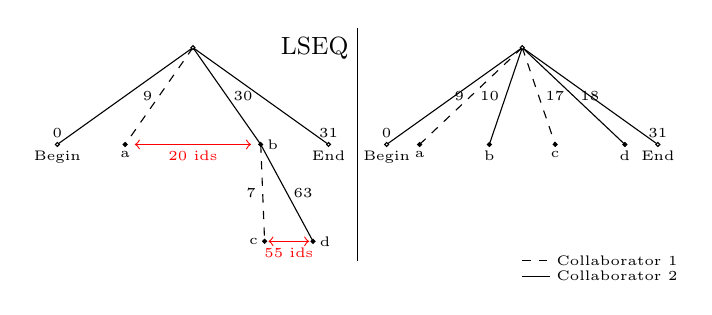
\begin{tikzpicture}[scale=0.7]
  \small

  \draw ( 85pt,10pt)node[anchor=north east]{LSEQ} node[anchor=north
  west]{\NAME{}}--( 85pt, -110pt);

  \tiny

  \draw (0,0) -- (-70pt, -50pt);
  \draw (0,0) -- ( 70pt, -50pt);

  \draw[dashed] (0,0) -- node[anchor=east]{9}  (-35pt, -50pt);
  \draw (0,0) -- node[anchor=west]{30} ( 35pt, -50pt);

  \draw[dashed] (35pt, -50pt) -- node[anchor=east]{7} (37pt, -100pt);
  \draw (35pt, -50pt) -- node[anchor=west]{63} (62pt, -100pt);

  \draw[fill=white] (0,0) circle (1pt);

  \draw[fill=white] (-70pt, -50pt) node[anchor=north]{Begin}
  node[anchor=south]{0} circle (1pt);

  \draw[fill=white] ( 70pt, -50pt) node[anchor=north]{End}
  node[anchor=south]{31} circle (1pt);

  \draw[fill=black] (-35pt, -50pt) node[anchor=north]{\ELEM{a}} circle (1pt);
  \draw[fill=black] ( 35pt, -50pt) node[anchor=west]{\ELEM{b}} circle (1pt);

  \filldraw[black] (37pt, -100pt) node[anchor=east]{\ELEM{c}} circle (1pt);
  \filldraw[black] (62pt, -100pt) node[anchor=west]{\ELEM{d}} circle (1pt);

  \draw[<->,color=red] (-30pt,-50pt) -- node[anchor=north]{20 ids}
  (30pt,-50pt);
  
  \draw[<->,color=red] (39pt,-100pt) -- node[anchor=north]{55 ids}
  (60pt,-100pt);

%% % % % %  %% %%% %% % % % % % %% % % % %%% %
  
  \draw (170pt,0pt) -- ( 100pt,-50pt);
  \draw (170pt,0pt) -- ( 240pt,-50pt);

  \draw[dashed] (170pt,0pt)--node[anchor=east]{9}(117pt,-50pt);
  \draw (170pt, 0pt)--node[anchor=east]{10}  (153pt,-50pt);
  \draw[dashed] (170pt, 0pt)-- node[anchor=west]{17} (187pt,-50pt);
  \draw (170pt, 0pt) --node[anchor=west]{18} (223pt,-50pt);

  \draw[fill=white] (170pt,0) circle (1pt);

  \draw[fill=white] (100pt,-50pt)node[anchor=north]{Begin}
  node[anchor=south]{0} circle(1pt);

  \draw[fill=white] (240pt,-50pt)node[anchor=north]{End}
  node[anchor=south]{31}circle(1pt);



  \draw[fill=black] (117pt,-50pt) node[anchor=north]{\ELEM{a}} circle (1pt);
  \draw[fill=black] (153pt,-50pt) node[anchor=north]{\ELEM{b}} circle (1pt);
  \draw[fill=black] (187pt,-50pt) node[anchor=north]{\ELEM{c}} circle (1pt);
  \draw[fill=black] (223pt,-50pt) node[anchor=north]{\ELEM{d}} circle (1pt);

  \begin{scope}[shift={(170pt,-110pt)}]
    \draw[dashed] (0,0) -- (0.5,0) node[right]{Collaborator 1};
    \draw[yshift=-\baselineskip-2pt] (0,0) -- (0.5,0) node[right]{Collaborator
      2};
  \end{scope}  

\end{tikzpicture}

%%% Local Variables: 
%%% mode: latex
%%% TeX-master: "../dchanges"
%%% End: 

\caption{Representation of the underlying exponential tree model of LSEQ and
  \NAME{}. Two collaborators insert two elements at the end of the document in
  order to get the sequence ``abcd''. On the random side, the collaborators
  employ antagonist strategies. On the hash side, the collaborators use the
  same allocation strategy. Both sides draw the same random numbers.}
\label{fig:hashexample}
\end{center}
\end{figure}

Figure~\ref{fig:hashexample} highlights the differences between the original
random strategy choice and our hash strategy choice. Both cases present two
collaborators inserting 2 elements one after the other. The expected result is
the sequence ``abcd''. Hence, Collaborator 1 generates the ``a'' and ``c'' and
Collaborator 2 generates the ``b'' and ``d''. In both cases they draw the
same numbers. However, in the case of random strategy choice, one collaborator
randomly chooses \emph{boundary+} twice while the other randomly chooses
\emph{boundary--} twice. When the editing behaviour is monotonic, the size of
identifiers quickly grows. On the opposite, the collaborators using \NAME{}
implicitly agree on using \emph{boundary+} at depth-1, consequently the
allocation follows the properties of one user edition presented
in~\cite{nedelec2013lseq}.

The next section aims to corroborate our assumptions by performing experiments
on different numbers of collaborators and by varying the latency of the
network.

%%% Local Variables: 
%%% mode: latex
%%% TeX-master: "../dchanges"
%%% End: 
